\documentclass{article}
\usepackage[utf8]{inputenc}
\usepackage{graphicx}
\usepackage{amsmath} % Required for the align environment

\title{Lab 1: Gradient Descent Implementation}
\author{2540002 - Nguyen Nhat Anh}
\date{May 2026}

\begin{document}

\maketitle
\newpage

\section{Introduction}
This report presents the code implementation and logical flow for the Gradient Descent laboratory work. It details the mathematical foundations and the iterative process used to optimize model parameters.

\section{Gradient Descent}
Gradient Descent is an iterative optimization algorithm used to minimize a cost function by adjusting model parameters in the direction of the steepest descent. It identifies optimal weights and biases by gradually reducing the error between predicted and actual outputs.

\begin{align}
\text{Cost function: } J(\theta_0, \theta_1) &= \frac{1}{2m} \sum_{i=1}^{m} \left[(\theta_0 + \theta_1 x^{(i)}) - y^{(i)}\right]^2 \\[10pt]
\frac{\partial J}{\partial \theta_0} &= \frac{1}{m} \sum_{i=1}^{m} \left((\theta_0 + \theta_1 x^{(i)}) - y^{(i)}\right) \\[10pt]
\frac{\partial J}{\partial \theta_1} &= \frac{1}{m} \sum_{i=1}^{m} \left((\theta_0 + \theta_1 x^{(i)}) - y^{(i)}\right) x^{(i)}
\end{align}

\newpage
\section{Implementation}
The implementation follows the logic flow illustrated below:

\begin{figure}[h]
    \centering
    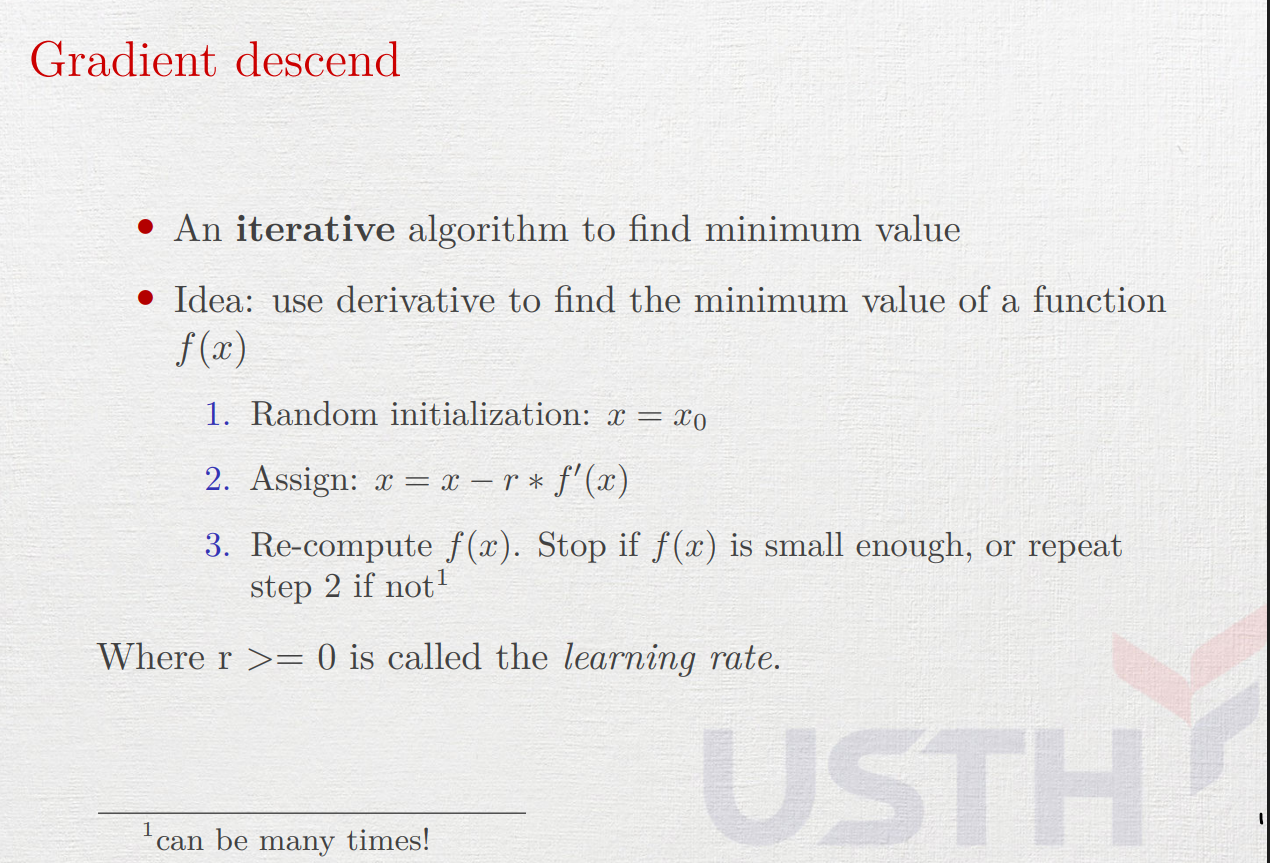
\includegraphics[width=0.8\textwidth]{grad_desc_flow.png}
    \caption{Gradient Descent Logic Flow}
    \label{fig:logic_flow}
\end{figure}

The function is designed using three primary parameters:
\begin{itemize}
    \item \textbf{Learning rate:} Determines the size of the steps taken toward the minimum.
    \item \textbf{Threshold value:} The convergence criteria to stop the iterations.
    \item \textbf{Initial x value:} The starting point for the optimization.
\end{itemize}

\newpage
\section{Results}
The output of the implementation is shown in Figure \ref{fig:output_result}:

\begin{figure}[h]
    \centering
    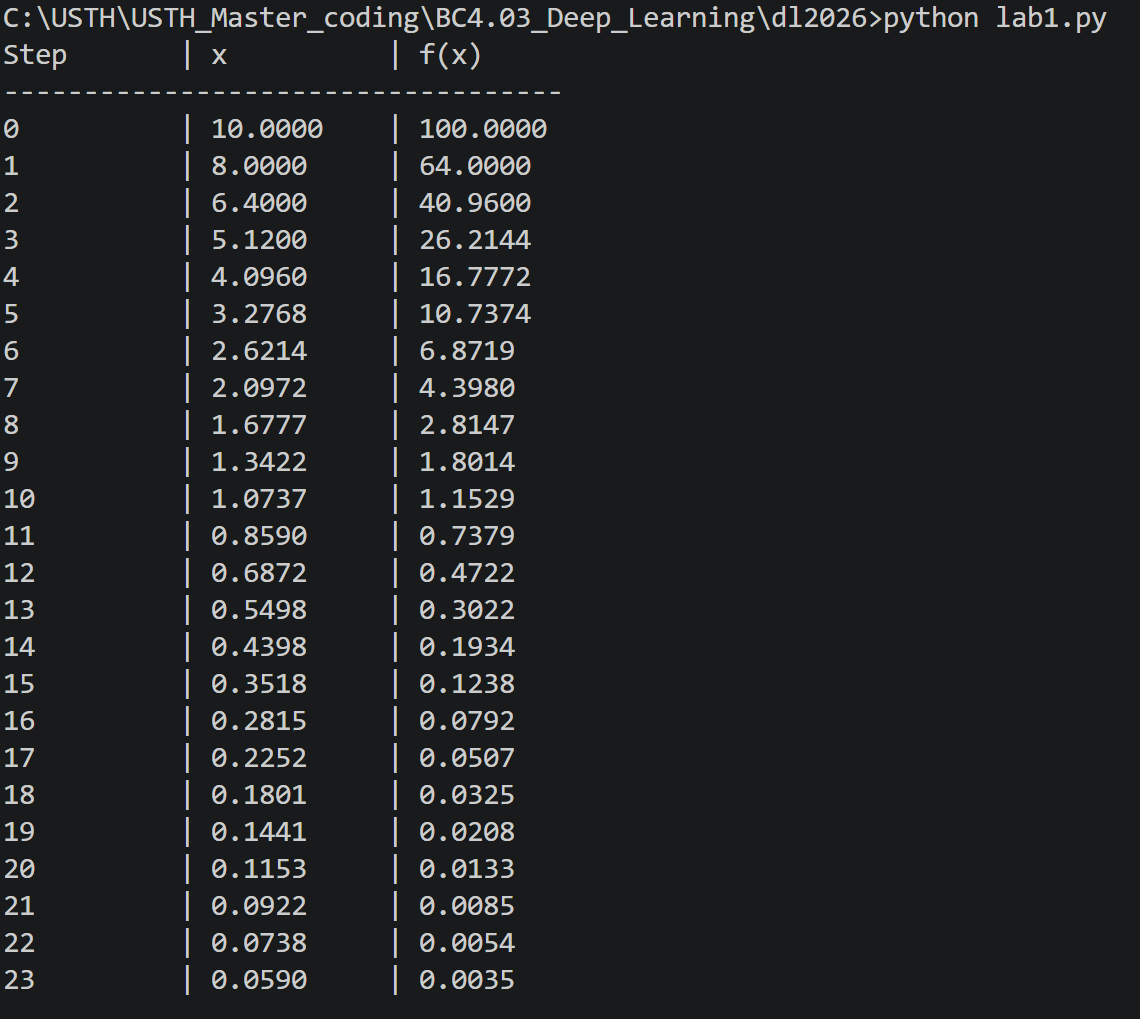
\includegraphics[width=0.75\textwidth]{output.png}
    \caption{Gradient Descent Output and Convergence}
    \label{fig:output_result}
\end{figure}

\end{document}